\section{Data Analysis}\label{anal.sec}

The data acquisition system used for E03-103, was the CODA (CEBAF Online Data
Acquisition) software package. CODA events from the individual run files were
decoded by the standard Hall C replay software. It reads the raw data written
by the data acquisition system, decodes the detector hits, locates possible
tracks and particle identification information for each event, and calculates
different physics variables. Input and output of the ENGINE are handled using
the CEBAF Test Package (CTP). ENGINE makes use of CERN HBOOK libraries and
provides output as ASCII report files (scalers, integrated charge $\ldots$),
histogram files (ADC/TDC spectra for different detectors) and the
reconstructed event-by-event data as ntuples. Detailed cuts, corrections and
other analysis details will be discussed in the following sections.



\subsection{Methodology of Cross Section Extraction}\label{proc.ssec}

The measured inclusive electron scattering cross section at scattered electron
energy $E^{\prime}$ and a central angle $\theta_{c}$ is extracted using
%
\begin{equation}\label{csmaster1.eq}
 \sigma^{Born}_{data}(E^{\prime},\theta_{c}) = \frac{Y_{data}}{Y_{sim}}\, \sigma^{Born}_{model}(E^{\prime},\theta_{c})
\end{equation}
%
where $\sigma^{Born}_{data}(E^{\prime},\theta_{c}) $ denotes the differential
cross section $\frac{d^2\sigma(E^{\prime},\theta_{c})}{dE^{\prime}d\Omega}$,
$Y_{sim}$ represents the simulated yield which includes the features of the
detector acceptance and the model radiated cross section, $Y_{data}$ is the
charge normalized yield integrated over the acceptance of the experiment and
$\sigma^{Born}_{model}(E^{\prime},\theta_{c})$ represents the Born model cross
section.  To the extent that the simulation properly includes the corrections,
efficiencies, and acceptance, the ratio of experimental yield to simulated yield
will simply reflect the error in the initial cross section model.

$Y_{data}$ is simply the number of detected electrons, averaged over the
kinematics, divided by the efficiency- and deadtime-corrected luminosity of the
measurement, so that $Y_{data}$ represents the normalized yield for an ideal
detector averaged over the acceptance of the experiment. The calculation of
$Y_{sim}$ must yields the same acceptance-averaged normalized yield,
and so must include a detailed model of the acceptance as well as all of the
physics effects required to go from the starting Born cross section model to
the final observed counts, i.e. radiative correction, multiple scattering,
energy loss, etc.... In addition, because this is the integrated yield over
the acceptance, the cross section model must do a reasonable job of accounting
for the cross section variation across the acceptance. Note that the
\textit{position-dependent} inefficiencies are applied to the simulation,
rather than the data, as discussed in Sec.~\ref{cercut.sssec}, and that
while the energy loss is included event-by-event in the simulation, a nominal
correction for the median energy loss is applied to both the data and
simulation to remove the average kinematic offsets.



\subsubsection{Extraction of experimental yield}\label{datayield.sssec}

Each kinematic setting contains data taken over one or more runs. Each run is
analyzed separately, with detector and acceptance cuts applied and the
efficiency and other experimental correction factors calculated run-by-run.
The efficiency-corrected and charge-normalized yield for all the runs in a
given setting, with
%
\begin{equation}\label{ydata.eq}
Y^{tot}_{data}=\frac{\sum_i N(i)}{N_{sc}~\sum_i C_{data}(i) \,Q_{tot}(i) },
\end{equation}
%
where $N_i$ is the total number of events which passes all cuts for $i^{th}$
run in the given setting, $Q_{tot}(i)$ is the total accumulated charge and
$N_{sc}$ is the number of scattering centers in the target; $N_{sc}=\rho t
N_A/M$ where $\rho$ is the density, $t$ is the thickness, $M$ is the atomic
mass of the target and $N_A$ is Avogadro's number. The factor $C_{data}(i) $
in Eq.~\ref{ydata.eq} is the correction factor which includes experimental
efficiencies and live times; $C_{data} = PS/(\varepsilon_{trig} \times
\varepsilon_{track} \times \varepsilon_{det} \times t_{comp} \times t_{elec})$
where PS is the prescale factor used to reduce the trigger rate when the data
is taken, $\varepsilon_{trig}$ corrects for the events lost due to
inefficiency at the trigger level, $\varepsilon_{track}$ is the tracking
efficiency, $\varepsilon_{det}$ denotes the global detector efficiencies, and
$t_{comp}$ and $ t_{elec}$ are the computer and electronic live time,
respectively.

Because we are only interested in primary beam electrons which scatter
in the target, we have to subtract the contribution of electrons which
scatter in the target entrance and exit windows (for the cryogenic targets)
and secondary electrons which come from other processes. The subtraction of
the cryotarget endcap contribution is discussed in Sec.~\ref{bg.sssec}, and the
secondary electrons in Sec.~\ref{csbg.sssec}.

\subsubsection{Extraction of simulated yield}\label{simyield.sssec}

In order to evaluate $Y_{sim}$ one needs to account for the finite acceptance
of the HMS using a detailed model of the spectrometer acceptance. Cuts
are applied to the measured and simulated distributions to limit the data to
events where the momentum acceptance is well understood.  These cuts, given in
Table~\ref{acccuts.tab} are large enough in angle so that the collimator
defines the angular acceptance, but are effective in removing in-scattering
events which reconstruct to trajectories outside of the acceptance.

\begin{table}[htb]
\caption{Acceptance cuts used in the analysis for data and simulation. Here,
$\delta$ is the relative deviation from the central momentum and $x'_{tar}$
and $y'_{tar}$ are the out-of-plane and in-plane angles of the reconstructed
tracks.}

 \begin{center}
 \begin{tabular}{|l|c|}
	 \hline
	 Variable & cut value \\
	 \hline
 abs($\delta$) & $<$~9\% \\
 abs($x'_{tar}$) & $<$~120 mrad\\
 abs($y'_{tar}$) & $<$~40 mrad \\
	 \hline
 \end{tabular}
 \end{center}
\label{acccuts.tab}
\end{table}

An acceptance function is generated and applied to the simulation to account
for the finite acceptance of the spectrometer. This function is
defined to be the probability that the spectrometer will accept an event
originating from a point in the target $(x_{tar},y_{tar}, z_{tar})$ with
momentum and angles described by three spectrometer coordinates $\delta,x^{'},
y^{'}$. In general, the acceptance is a function of the six variables
$(\delta, x^{'}, y^{'}, x_{tar}, y_{tar}, z_{tar})$ that fully define the
event, and is generated by Monte Carlo. It is not feasible to generate the
full six-dimensional acceptance function, but it can be simplified by
integrating over variables.  Because the yield is the acceptance-weighted
cross section, we can average over variables which do not impact the cross
section or which are uniformly populated. Since there is no significant loss
of beam intensity along the target, the distribution in $z_{tar}$ is uniform,
so the acceptance function can be integrated over $z_{tar}$. Similarly, we do
not bin in the target $x$ or $y$ positions, and so we can integrate the
acceptance function over a range in target position that corresponds to the
observed position and raster size of the beam. Note that while we do not bin
the data in the target position variables, we do use the reconstructed
vertical target position to calculate a small correction to the reconstructed
momentum of the event in both the data and simulation. This yields an
acceptance function that depends only on the trajectory of the event at the
target, $A(\delta, x^\prime, y^\prime)$, the same subset of target variables
that go into the cross section model. If instead we write the acceptance and
cross section as a function of the scattering angle, $\theta$, and azimuthal
angle, $\phi$, the inclusive cross section depends only on $E^\prime$ and
$\theta$, and so the acceptance function can be integrated over $\phi$,
yielding a two-dimensional acceptance function. The acceptance function is
then calculated using a realistic distribution of event positions in the
target, meaning that it must be calculated separately for each effective
target length as seen by the spectrometer, i.e. separate for point-like and
extended targets, and for each different spectrometer scattering angle.


The final yield is an integral of the acceptance function over the
phase space, weighted by the differential cross section:
%
%\begin{eqnarray}
% Y_{sim} &= \int dE^{\prime} d\theta ~ \varepsilon^{\prime}_{det} ~
% A(\delta, x^{'}, y^{'}, x_{tar}, y_{tar}, z_{tar}) \nonumber \\
% &{}\sigma^{rad}_{model}(E^{\prime},\theta,\phi) ~,
%\end{eqnarray}
%
\begin{equation}
 Y_{sim} = \int dE^{\prime} d\theta ~ \varepsilon^{\prime}_{det} ~
 A(E^{\prime},\theta) {}\sigma^{rad}_{model}(E^{\prime},\theta,\phi) ~,
\label{simy.eq}
\end{equation}
%
where $\varepsilon^{\prime}_{det}$ accounts for any position-dependent
efficiencies in the detectors and $\sigma^{rad}_{model}$ is the cross section
model, including radiative effects. 

%\begin{equation}
% Y_{sim} = \int dE^{\prime} d\theta ~ \varepsilon^{\prime}_{det} ~
% A(E^\prime, \theta) ~ \sigma^{rad}_{model}(E^{\prime}, \theta) ~,
%\label{simy.eq}
%\end{equation}



The Hall C single arm Monte Carlo was used for the acceptance calculation.
Each event is randomly generated in the target coordinates, while the
quantities $\delta, y^{'}, x^{'}$ are randomly chosen within their allowed
limits. Then the particles are projected forward and transported to the
detector hut using transport matrix elements calculated by the COSY INFINITY
program~\cite{berz_cosy}, which models magnetic transport properties of the
spectrometer. Events that fail to pass through the different apertures defined
in the model are rejected.  Multiple scattering is simulated as the electrons
pass through material in the spectrometer, and so the acceptance function
is generated for each spectrometer momentum setting to account for the
energy-dependence of the scattering. If the particle successfully traverses the
spectrometer and passes all the criteria in the detector then it is accepted.


After applying cuts and binning the Monte Carlo counts in the same manner as
data, the acceptance function is simply the fraction of events in
a given bin that were accepted and passed all cuts. The integral in
Eq.~\ref{simy.eq} is evaluated in each bin, Thus the weighted, simulated yield
in Eq.~\ref{simy.eq} for a particular $(E^{\prime},\theta)$ bin is given by
%
\begin{equation}
Y_{sim} (E^{\prime},\theta)= \sum_{events} \varepsilon^{\prime}_{det}\sigma^{rad}_{model}(E^{\prime},\theta)~(\Delta E^{\prime}\Delta \Omega)_{bin}
\end{equation}
%
where $(\Delta E^{\prime}\Delta \Omega)_{bin}=(\Delta E^{\prime}\Delta
\Omega)_{bin}^{gen}/(N_{bin}^{gen})$ represents the relative phase space for a
given event in the bin. The generated solid angle depends on the generation
limits in $x^{'}_{tar}$ and $y^{'}_{tar}$. In this analysis $5\times 10^{6}$
events were generated for each simulated ntuple with generation limits
$\delta=\pm 15\%$, $x^{'}_{tar}=\pm 100~mr$ and $y^{'}_{tar}=\pm 50~mr$.
Once the measured and simulated yields yield have been obtained, the yield
ratio is applied as a correction factor to the initial Born cross section used
in the simulation to extract the final cross sections (Eq.~\ref{csmaster1.eq}).

\subsection{Efficiencies}

In the cross section analysis, we apply particle identification (PID) cuts on
the signals from the gas $\mathrm{\check{C}erenkov}$ counter and lead-glass
calorimeter to distinguish electrons from other negatively charged particles.
Because of this, we must also correct for losses of real events when these
cuts are applied arising from detector-related inefficiencies. There are
additional losses due to trigger inefficiency or inefficiency of tracking
algorithm to find a valid track.  Finally, the calorimeter and
$\mathrm{\check{C}erenkov}$ detectors are used to reject pions, and the 
pion rejection cuts can yield a small electron inefficiency.

\subsubsection{Trigger efficiency}\label{trigeff.sssec}

The trigger was designed to be efficient for electrons while suppressing other
particle types. The electron trigger is described in detail
elsewhere~\cite{blok08, johna_thesis, aji_thesis}, and the key points are
summarized here. There are two main electron triggers. The first requires
signals from 3/4 hodoscope layers and a signal from the calorimeter. 
The second requires a $\mathrm{\check{C}erenkov}$ signal and either 3/4
hodoscope planes or 2/4 planes (one from the front and one from the back) and a
calorimeter signal with a lower threshold than the other trigger. This way,
even if the $\mathrm{\check{C}erenkov}$ or calorimeter have low efficiency, or
the 3/4 hodoscope efficiency falls, we still maintain a high trigger
efficiency based on the other two detectors.

Because there were no problems with the operation of the detectors, the
final trigger level efficiency was extremely high. The efficiency for
a good event to give signals in 3 of the 4 hodoscope planes was determined
run-by-run, and found to be 99.2\% on average.  The efficiency for the 
time-of-flight trigger (two planes, one in front, one in back) was 99.7\%.
While the time-of-flight trigger required both a signal from the calorimeter
and Cerenkov detectors, the 3/4 required only one PID signal, making the
trigger efficiency high even if one of the detectors had a low efficiency.
Accounting for all of these effects, the trigger efficiency is
99.7\%~\cite{aji_thesis}, and was largely rate and kinematic independent,
yielding a negligible uncertainty in the cross section ratios.


\subsubsection{Tracking efficiency}\label{track.sssec}

The normalized yields must also be corrected for inefficiencies in the
tracking. The tracking efficiency is defined as the fraction of good events
which yield a valid track. A track can be lost to hardware inefficiency or
failure in the tracking algorithm, often due to missing planes or excess
noise or background hits. The tracking efficiency correction was applied on a
run-by-run basis. At low rates, the efficiency was approximately 98\%, with a
small reduction at high rates (up to 2\%) which is consistent with the
expected loss due to rejection of events with real multiple tracks.


\subsubsection{Calorimeter cut efficiency}\label{caloricut.sssec}

To reject pions, we require that the energy deposited in the calorimeter be at
least 70\% of the reconstructed momentum ($E_{cal}/E^{'}$$>$0.7).  It is
important to know how many otherwise valid events are lost when we place a cut
on the calorimeter distribution. To determine the fraction of electrons lost
due to the calorimeter cut, we need to identify a clean and unbiased sample of
electrons.  For this analysis, we used elastic scattering data, where the
initial fraction of pions is small, and then apply a cut on
$\mathrm{\check{C}erenkov}$ detector to yield a pure electron sample. While
elastically scattered electrons tend to populate a limited region in the
acceptance of the spectrometer, this region can be moved across the acceptance
by changing either the angle or scattered electron momentum, allowing us to
map out the response of the spectrometer throughout the acceptance. We use
these scans to verify that the cut efficiency is uniform across the
acceptance. The efficiency is found to be constant for $E^\prime$ above 1.7
GeV ($99.89\%$), but below this momentum, the efficiency starts to decrease
mainly due to decreasing resolution of the calorimeter. This falloff is
approximately linear, dropping the efficiency by 0.3\% for $E^\prime \approx
0.7$~GeV/c~\cite{aji_thesis} and is parameterized as a function of the
scattered electron momentum and is used to correct data in the analysis. The
efficiency measured with elastics is consistent with the efficiency extracted
using inelastic kinematics which populate the full acceptance, where the
kinematics have few enough pions for the $\mathrm{\check{C}erenkov}$ to yield
a pure electron sample.


\subsubsection{Cerenkov cut efficiency}\label{cercut.sssec}

Another cut was applied on the number of photo-electrons collected by the
$\mathrm{\check{C}erenkov}$ detector in order to distinguish electrons from
pions. In addition to the pion-rejection cut in the calorimeter, we also
require the $\mathrm{\check{C}erenkov}$ detector sees at least 1.5
photo-electrons.  To measure the electron efficiency of this cut, we
generate a pure sample of electrons using elastic scattering kinematics
along with a cut on the calorimeter.

During the analysis it was found that the signal from the
$\mathrm{\check{C}erenkov}$ detector was lower near the vertical center of the
detectors, corresponding to $\delta =0$.  This is due to the gap between the
upper and lower mirrors. In addition to this $\delta$-dependent inefficiency,
the $\mathrm{\check{C}erenkov}$ has a momentum-dependent inefficiency due to
variation of $\mathrm{\check{C}erenkov}$ cone with particle momentum. The
efficiency was parameterized in terms of both $\delta$ and the HMS momentum
setting. The efficiency is close to 100\% for momenta above the central
momentum setting, 1--2\% lower on the low-momentum side of the acceptance,
with loss of up to 2--4\% efficiency in the central $\pm$0.5\% of the momentum
acceptance (the inefficiencies are larger at low momentum settings).  For
details, see Ref.~\cite{aji_thesis}.


\subsection{Backgrounds}\label{bg.ssec}

In addition to the scattered electrons, there are secondary electrons that are
in the acceptance of the detector due to other physical processes which
constitute a background for the measurement. This background mainly consists
of scattered electrons from the cryotarget cell wall, pions that survive the
nominal PID cuts and are treated as scattered electrons, and secondary
electrons from pair production after bremsstrahlung in the target or $\pi^0$
which decay to photons. The following subsections discuss each of these
processes, and how we estimate and correct for them in the analysis.
 
\subsubsection{Background from target cell wall}\label{bg.sssec}
Since the cryogenic targets were contained in aluminum cells, electrons
scattered from the cell walls also contribute to the total number of detected
events. This contribution is measured and subtracted from the total
detected events. The cryocells were made of Al 7075 which has a density of
2.7952~g/cm$^3$ and the thickness of the cell walls was $\sim$0.12~mm. The
electrons traverse two cell walls, and since the cryotarget thickness varies
between 0.2 to 0.6~g/cm$^2$, the typical size of the background contribution
is between $10\%$ to $20\%$. We used a dummy aluminum target to directly
measure the cell wall contribution to the total yield. The dummy target
consists of two Al foils (Al 6061- T6) separated by $\sim$4~cm which are
$\sim$8 times thicker than the cryocell walls, thus allowing a higher
luminosity and a smaller data acquisition time. During the experiment dummy
data were taken at the same kinematics as the cryotarget data. Dummy data are
treated in the same way as cryotarget data and the normalized dummy yield is
subtracted from the cryotarget yield. Thus the total yield is
%
\begin{equation}
Y = Y_{cryo}- \left[ \frac{R^{ext}_{dummy}}{R^{ext}_{walls}}\,
\frac{T_{walls}}{T_{dummy}} \right] \times Y_{dummy},
\end{equation}
%
where $T_{walls}$ and $T_{dummy}$ are the thicknesses of the cell walls and the
dummy respectively, $Y_{e}$ and $Y_{ed}$ are the measured cryotarget yield and
dummy yield respectively, and the ratio of $R^{ext}_{dummy}$ and
$R^{ext}_{walls}$ represents a correction factor which is applied to the
radiative corrections of the dummy yields. This correction factor is due to
the difference in thickness between dummy and the cryotargets which modifies
the external bremsstrahlung. The correction was found to be about 5\% for
larger scattering angles at low $x$ values and smaller for other angles.


\subsubsection{Charge symmetric  background (CSB)}\label{csbg.sssec}

At low $x$ and high $Q^2$, there is a significant probability that the
incident electron can interact with the target nuclei and produce neutral
pions in the target. These pions can decay into high energy photons which
produce an equal number of positrons and electrons. The total number of
electrons detected in the spectrometer is $e^-_{detected} = e^-_{primary} +
e^-_{background}$. Since an equal number of positrons and electrons are
produced, the yield is charge symmetric. This allows us to estimate the number
of secondary background electrons by running the spectrometer with positive
polarity and detecting the positrons. During E03-103, we used the HMS to take
positron data for each target at all kinematics setting where the CSB was
significant, allowing for a direct subtraction of the background by assuming
$e^-_{background} =e^+_{detected}$.  Luminosity normalized yields are used
to subtract the CSB, with identical cuts applied to the positron and electron
data.
%
%\begin{equation}
%\label{csb_eqn}
%R_{csb} =\frac{ Y_{e^+}}{Y_{e^-}} = \frac{Y_{background}}{Y_{scattered}+Y_{background}}
%\end{equation}
%
%where $Y_{e^-}$, contains the total yield from primary scattered electrons and
%the background.
%
$R_{csb}$, the fraction of the detected electrons associated with CSB,
is shown in Fig.~\ref{csbg_fig} as a function of $x$ for the 50 and 40 degree
data. Note that our final EMC ratios are formed from the 40 degree data, and
so the correction is below 10\% except for the smallest values of $x$ and the
high-$Z$ targets.

%-------------------------------------
\begin{figure}[htb]
\begin{center}
\includegraphics[width=80mm,angle=0]{plots/50deg_csbg_mod.eps}
\includegraphics[width=80mm,angle=0]{plots/40deg_csbg_mod.eps}
\caption{The charge symmetric background as a function of $x$ for data taken
at 50 degrees (top) and 40 degrees (bottom).
\label{csbg_fig}}
\end{center}
\end{figure}
%------------------------------------

\subsubsection{Pion backgrounds}\label{picont.sssec}

Pion rejection factors for the $\mathrm{\check{C}erenkov}$ and calorimeter
detectors are always greater than 500:1 and 100:1, respectively.  Nonetheless,
for runs with a high $\pi/e$ ratio, there could still be a small contamination
of pions after the PID cuts.

%However, some pions can fire the $\mathrm{\check{C}erenkov}$ detector by
%producing knock-on electrons in the aluminum entrance window. These knock-on
%electrons are of high enough energy to emit $\mathrm{\check{C}erenkov}$ light
%and will pass the nominal $\mathrm{\check{C}erenkov}$ cut.
%
%As mentioned earlier, pions in the calorimeter give a signal corresponding to
%their energy loss which is on average 0.3 GeV/$E^{'}$. However, through a
%charge exchange reaction they can produce neutral pions, which decay into two
%photons. Thus, the full energy of a $\pi^0$ can be deposited in the
%calorimeter, and this will show up as a high energy tail in the calorimeter
%spectrum that extends well beyond the cut at 0.7.

To estimate the pion background for high $\pi/e$ kinematics, we generate
calorimeter spectra for electron runs (including all of the PID cuts except
the software calorimeter cut), and pure pion spectra (using runs without
trigger-level PID and requiring less then 0.5 photo-electrons in the
$\mathrm{\check{C}erenkov}$.  The pion sample is renormalized to match the
pion background in the `electron' sample at $E_{cal}/E^{\prime}$$<$0.7, and
the tail of the pion spectrum extending to $E_{cal}/E^{\prime}$$>$0.7 is
used to estimate the pion contamination after all PID cuts. It was found that
the final pion contamination is always below $0.5\%$.  This is further
suppressed as the subtraction of the positive-polarity data intended to remove
charge-symmetric backgrounds (see section ~\ref{csbg.sssec}) will have a
nearly identical contribution from positive pions.  We estimate that any
residual pion contamination is extremely small, and so we do not apply any
correction, but assign a 0.2\% point-to-point uncertainty to
allow for a small net contribution of pions.


\subsection{Target boiling corrections}\label{tarboil.ssec}
When the electron beam passes through the target material of cryogenic
targets, it deposits energy in the form of heat. This causes local density
fluctuations, ``target boiling'', along the path of the beam. The boiling
effects depend on the beam current, beam raster size and the thermal
properties of targets. We perform luminosity scans, measurements of the yield
at fixed kinematics with varying beam currents, to estimate the boiling
effects. In addition to measuring the effect on the cryogenic targets, we also
take data on carbon as a reference measurement, to insure that corrections for
rate-dependent effects do not introduce variations which are misinterpreted as
density fluctuations.

A small current dependence was observed for the carbon target, even after
correcting for all known rate-dependent effects. Because the beam-current
monitors have an uncertainty in their DC offset, an error in that offset can
yield an error in the charge that goes like the inverse of the beam current.
The effect in carbon was small enough to be consistent with the uncertainty
in the BCM offset uncertainty, and so the current dependence in the cryogenic
targets were taken relative to the carbon results to remove this effect. The
hydrogen and deuterium targets did not show any residual slope after
correcting for the BCM offset, but the helium targets show a linear drop in
the yield. For $^{3}$He, the measured density loss was $(-3.10 \pm 0.64)\% $ at
$100\,\mu A$ and for $^{4}$He, $(-1.27 \pm 0.50)\% $ at $100\,\mu A$. The
yield for each run is divided by a correction factor which depends linearly on
the average current (excluding periods with no beam).

% stuff about dead times
\subsection{Computer and electronics deadtimes}

Events are also lost due to the finite time it takes to either form a trigger
for an event or read out the data. During the time the trigger or
DAQ systems are busy, no new events can be taken. This is monitored on a
run-by-run basis by looking at the number of events generated with final
trigger module widths of 50, 100, 150 and 200~ns, and the electronic deadtime
scales with the trigger rate and gate width except for the 50~ns measurement.
While the typical gate widths are 40~ns, the coincidences formed between
different hodoscope planes have variable widths, typically 50-60~ns, so our
final trigger module is set to 60~ns to minimize the event-to-event variation
of the effective latency time. We calculate and apply a deadtime correction of
60~ns time the raw pretrigger rate, yielding a maximum correction of 1.5\%,
but typical values well below 0.5\%.


Computer deadtime occurs when the DAQ computers are busy processing events
(either digitizing fastbus information or sending the data to the DAQ
computers), and are not available for processing new events. Because the
events are buffered in the fastbus and VME modules, there is not a fixed
latency period for each event, so we make a direct measurement of the
computer deadtime and apply the correction on a run-by-run basis. We take
the number of events recorded to disk divided by the number of generated
triggers which should have been read out and take the ratio to be the live
time. The deadtimes were kept below 20\% by adjusting the prescale factors,
although previous tests have shown reliable operation and corrections for
deadtimes well over 90\%~\cite{johna_thesis}.


\subsection{Cross Section Model}\label{modelxsec_sec}

A cross section model is required for the bin centering corrections, the
radiative corrections and the Coulomb corrections. The Born cross section
model (known as XEM model) is broken down into contributions from inelastic
and quasielastic scattering:
%
\begin{equation}
\label{Bornmodel_eqn}
\sigma_{Born} =\sigma_{inel} + \sigma_{qe} ~.
\end{equation}

For the quasi-elastic contribution $\sigma_{qe}$, we use a $y$-scaling model.
The scaling variable $y$ can be interpreted as the minimum momentum of the
struck nucleon in the direction of the virtual photon. The scaling function,
$F(y)$, is an energy and momentum integral of the spectral function and is
defined as the ratio of the measured nuclear cross section to the off-shell
cross section for a nucleon, multiplied by a kinematic
factor~\cite{day_fymodel, johna_thesis, nadia_thesis}:
%
\begin{equation}
\label{Fy_eqn}
F(y) = \frac{d\sigma}{d\Omega d\nu}\frac{1}{\mathrm{Z}\sigma_p +
\mathrm{N}\sigma_N} \frac{q}{\sqrt{M^2 +(y+q)^2}},
\end{equation}
%
where Z is the number of protons in the nucleus, N is the number of neutrons,
$q$ is the three-momentum transfer, and $M$ is the proton mass. $F(y)$ is
expected to scale in $y$ on the low energy loss side of the quasielastic peak
where inelastic contributions and final state interactions are minimal. The
scaling function used for \LD\, is from~\cite{Mckeown_fymodel} and has the
form:
%
\begin{equation}
\label{Fy_eqn2}
F(y) =(f_0-B) \frac{\alpha^2\, e^{-(ay)^2}}{\alpha^2+y^2} + B \, e^{-b|y|}.
\end{equation}
%
For heavier targets this was modified to be:
%
\begin{equation}
\label{Fy_eqn3}
 F(y) =(f_0-B) \frac{\alpha^2\, e^{-(ay)^2}}{\alpha^2+y^2} + B \, e^{-(by)^2},
\end{equation}
%
where the parameters $a, b, f_0, B $ and $\alpha$ are fit to the $F(y)$,
extracted from the data for each target.  The model parameters were varied
to reproduce the data from this measurement, along with the measurements
covering $x \gtorder 1$ on the same targets from Refs.~\ref{fomin10,fomin12}.
The model was also compared to low $Q^2$ quasielastic data, taken from
Ref.~\cite{Benhar:qe_archive}, because of the importance of events from low
$Q^2$ quasielastic scattering, which has a large cross section, radiating
down into the lower $x$ kinematics for this experiment.

%In the partial wave impulse
%approximation of quasi elastic scattering, the extracted scaling function
%$F(y)$ can be related to the nucleon momentum distribution via
%%
%\begin{equation}
%\label{Fy_nucmom_eqn}
%F(y) = \int_{|y|}^{\infty} n(k)~k~ dk
%\end{equation}
%
%Thus with the knowledge of $F(y)$ one can extract the momentum distribution
%$n(k)$ and hence the nuclear structure functions using
%%
%\begin{equation}
%\label{F2a_eqn}
%F_2^A= \int |n(k)|^2 dk ~(Z F_2^p + (A-Z) F_2^n)
%\end{equation}
%%
%where $F_2^p$ and $F_2^n$ are proton and neutron structure functions
%respectively.

F(y) was extracted from the data in the QE region after subtracting the
inelastic contribution (calculated using the inelastic part of the
model)~\cite{nadia_thesis}. After fitting F(y), the updated model was used as
the input for the cross section extraction, and the process was repeated until
good agreement between data and the model was achieved for all settings. In
addition, an angle independent global polynomial correction was used for each
target to improve the agreement between data and model. 

%\textit{JRA: ************* Is that really what we do? Do we use the same
%F(y)/n(k) for the inelastic as we do for the QE? What about the normalization,
%which isn't unity for the QE (IIRC)? ****************}

For the deuteron, parameterizations of the proton and neutron structure
functions (developed by P. Bosted and E. Christy~\cite{bosted_model}) are used
for the full $x$ range. They are smeared using the momentum distribution based
on the fit to our QE peak~\cite{nadia_thesis}.

For heavier nuclei, the inelastic cross section is computed differently. For
$x<0.8$, the inelastic cross section is built from the $^2$H model using the
`inelastic' EMC ratio obtained from our data. These inelastic ratios
are obtained from the data by subtracting the quasi-elastic
model from the cross section; the subtraction is negligible at high $Q^2$, 
where we quote our EMC ratios, but is more important for the low $Q^2$ model.
For $x>0.9$, the smearing prescription is used with the corresponding momentum
distribution for each target, and a linear interpolation between the two
parts of the model is used between $x=0.8$ and 0.9.

The inelastic part of the model used for radiative correction is slightly
different from the model above. The inelastic model used for bin centering has
the disadvantage that, at low $Q^2$, the resonances do not get smeared out
enough, leaving some residual structure in the data to model ratios. For the
radiative corrections therefore it was decided to use the smearing
prescription for the full $x$ range. For $x<0.8$, the model is the sum of the
proton and neutron structure functions smeared by the momentum distribution.
For $x<0.8$, this inelastic model is then multiplied by a target-dependent
polynomial function to improve the agreement between data and model. This is
smoothly joined to the full smearing prescription for $x>0.9$, using an
$x$-weighted average for $0.8<x<0.9$. For the bin centering, we need the Born
cross section on a two dimensional grid in $\theta$ and $x$ (or $E^{'}$), and
the smearing prescription for the inelastic model cannot be used because of
the significant increase in CPU time. However, once the bin centering
corrections are applied, the data are centered to the central angle. Hence,
the radiative correction table can be one dimensional, since the data are
centered to the central angle of the setting. The data as well as the model
cross sections, including the relative contributions from the inelastic piece
and the quasielastic piece for $^2$H and $^{197}$Au are shown in
Fig.~\ref{all_model_compare_fig}.

%\textit{JRA: Not sure I understand this; have to double check thesis, see
%about rewording it to be a bit more clear. Also, have to be clear about 2
%models, one for RC, one for all other aspects (not just 'bin centering', which
%we don't do as a separate/formal step in any case.  WAITING TO UPDATE THIS
%UNTIL FINAL RC MODEL SORTED OUT.)}

%--------------------------------------
\begin{figure}[htbp]
\begin{center}
\includegraphics[width=80mm, angle=0]{plots/ld2_worldDM.eps}
\includegraphics[width=80mm, angle=0]{plots/au_worldDM.eps}
\caption{Comparison of world data from the
quasielastic electron nucleus scattering archive~\cite{Benhar:qe_archive} and
our cross section model for a variety $Q^2$ settings (average $Q^2$ values
quoted is for the quasielastic peak) for the $^2$H (top) and $^{197}$Au
targets. The shape of the QE peak is well reproduced for both targets
at both low and high $Q^2$, yielding a nearly flat ratio of data/model over
the entire $x$ range.
\label{all_worlddata_compare_fig}}
\end{center}
\end{figure}

%-------------------------------------------

At low $Q^2$ values, the quasi-elastic peak accounts for a significant portion
of the total cross section at large $x$.  The low-$Q^2$ QE cross section also
has a large impact on the radiated model at low $x$ and high $Q^2$. We have
done extensive studies and compared our model with the data available from the
quasielastic electron nucleus scattering archive~\cite{Benhar:qe_archive}. For
heavy nuclei, our model cross section was compared with world QE
data down to $Q^2=0.5$~GeV$^2$, and the agreement between data and model was
found to be at the 10\% level near the quasi-elastic peak, as shown in
Fig~\ref{all_worlddata_compare_fig}.

%--------------------------------------
\begin{figure}[htbp]
\begin{center}
\includegraphics[width=80mm, angle=0]{plots/ld2_model_example.eps}
\includegraphics[width=80mm, angle=0]{plots/au_model_example.eps}
\caption{Data and model cross section for $^2$H and $^{197}$Au at selected
kinematics. Here, the circles shows 18 degree data and the squares shows 50
degree data. Relative contribution from inelastic (dashed line) and
quasielastic (dotted line) to the total cross section (solid line) are also
shown in the figure.}\label{all_model_compare_fig}
\end{center}
\end{figure}
%-------------------------------------------

\subsection{Other corrections}\label{othercor.ssec}

%\begin{figure}[htb]
%\begin{center}
%\includegraphics[height=50mm,angle=0]{plots/radfigure1.eps}
%\caption{Lowest order Feynman diagrams for inclusive lepton-nucleon scattering.
%\textit{JRA: Not quite; multi-photon isn't lowest order}.\label{radcor_fig1}}
%\end{center}
%\end{figure}


The XEM cross section model is in the Born or one-photon exchange
approximation. However, higher order processes in $\alpha$ also contribute to
the measured cross sections~\cite{motsai_rc,tsai_rc} and must be applied to
the starting model. To compare to the measured cross sections, all significant
contributions from higher order processes must be estimated and corrected for
in the measured cross section. These include traditional radiative corrections,
as well as the ``Coulomb corrections'' associated with the long-range
interaction of the electron with the charge of the nucleus.


\subsection{Radiative corrections}\label{rc.ssec}


%For the external corrections, the incoming or outgoing electron radiates a
%real photon due to interactions with the fields of nuclei other than the
%target. This process depends on the the amount of material that the incident
%and scattered electron traverse including the target thickness. Among the
%external processes are external bremsstrahlung and ionization energy losses.
%Internal effects occur at scattering vertex, and are calculable in QED.
%Internal effects include internal bremsstrahlung, vacuum polarization, vertex
%correction and multiple photon exchange. Many of these processes involve
%modification of the kinematics at the scattering vertex, and in some cases the
%radiative corrections bring in large contributions from kinematic regions with
%a much larger cross section.

%
%\begin{figure}[htb] \begin{center}
%\includegraphics[height=25mm,angle=0]{plots/radcorfig2.eps} \caption{Different
%processes that can contribute to the measured cross
%sections for a nuclear target.
%\label{radcor_fig2}}
%\end{center}
%\end{figure}
%

Radiative corrections need to be applied to account for higher order QED
diagrams, the most significant of which are the emission of one or more
real photons by the incoming or outgoing electron or the struck quark (in the
DIS regime), exchange of a virtual photon between the incoming and outgoing
electron, and the fluctuation of the exchange photon into a lepton-antilepton
pair.  Because the elastic and quasielastic cross sections are very large
at low $Q^2$, one must also account for low-$Q^2$ interactions which, due to
radiation of a hard photon, end up at low $x$ and high $Q^2$ values.
Thus, we express the total radiated cross section as:
%
\begin{equation}
\sigma_{measured}= \sigma^{radiated}_{inelastic}+
\sigma^{radiated}_{quasielastic}+ \sigma^{radiated}_{elastic} ~.
\end{equation}
%
Since the inelastic radiative cross section is largely proportional to the
Born cross section for our kinematics ($>$80\%), we used the multiplicative
radiative correction method. For the kinematics of this analysis, our studies
indicate that the nuclear elastic tail contributes less than 0.1\% to the
total cross section for $^2$H, and significantly smaller contributions for
heavy nuclei, and so are neglected in the analysis.



%The radiative correction factor RC is
%%
%\begin{equation}
%RC=\frac{\sigma^{model}_{Born}}{\sigma^{model}_{radiated}},
%\end{equation}
%%
%where $\sigma^{model}_{Born}$ is the model cross section due to the exchange
%of a single photon and
%


The program used to compute the radiative corrections for this analysis was
developed at SLAC and is described in detail in~\cite{dasu_thesis}. For
E03-103, the external corrections are computed using a complete calculation of
Mo-Tsai~\cite{motsai_rc} with a few approximations. Note that, in particular,
the energy-peaking approximation is not used for the computation of external
contributions. This approach, ``MTEQUI'', uses the equivalent radiator
approximation~\cite{dasu_thesis}. In the equivalent radiator method, the
effect of ``internal'' Bremsstrahlung is calculated using two hypothetical
radiators of equal radiation length, one placed before and one after the
scattering. The internal contribution in ``MTEQUI'' method is evaluated by
setting the radiation length of the material before and after the scattering
point to zero, and ignoring the target length integral. Then the radiated
model cross section is given by the sum of the internal and external
contributions.


%\begin{equation}
%\sigma^{model}_{radiated}= \sigma^{int+ext}_{MTEQUI}
%\end{equation}


Our simulations are performed using the radiated model,
%
\begin{equation}
\label{rc1_eqn}
\sigma^{model}_{radiated}=external\otimes internal \otimes \sigma^{model}_{Born},
\end{equation}
%
is the model cross section due to the sum of all higher-order diagrams. The
convolution involves integrating over the ``internal'' and ``external''
bremsstrahlung photon momenta and angles, and the target dimensions.
To obtain $\sigma^{model}_{radiated}$, one needs to know the cross sections
over the entire kinematic range (from elastic threshold up to the kinematic
point being calculated, see Figure C.1 in reference~\cite{dasu_thesis}). The
effect of radiative correction on measured cross sections varied from a few
percent to about $40\%$, depending on the kinematics and targets. Because the
structure functions of nuclei are very similar, the internal radiative
corrections and some of the external corrections cancel, yielding smaller
corrections in the target ratios which depend mainly on the difference in the
targets radiation length, as shown in Fig.~\ref{rc_superrat_fig}.


%--------------------------------------
\begin{figure}[htbp]
\begin{center}
%\includegraphics[width=80mm, angle=0]{plots/50deg_rc_suprat.eps}
\includegraphics[width=80mm, angle=0]{plots/40deg_rc_suprat.eps}
\caption{Radiative correction factor to the A/D cross section ratios for a
range of targets at 40 degrees; the correction at 50 degrees is nearly
indistinguishable.
\label{rc_superrat_fig}}
\end{center}
\end{figure}
%-------------------------------------------

\subsection{Coulomb corrections}\label{cc.ssec}

The incoming electron will interact with the Coulomb field of the nucleus
prior to interacting with the nucleus. Classically, once the electron enters
the electron cloud of the atom, the screening of the nuclear potential is
no longer perfect, and the electron will be accelerated towards the nucleus,
increasing its momentum at the interaction vertex. After the scattering,
there will be a similar interaction as the electron leaves the nucleus.
This change in the kinematics can have a significant effect on the measured
cross sections if either the Coulomb potential is large compared to the energy
of the initial or final electron, or when the cross section varies rapidly
with the kinematics. In addition to the modification of the scattering
kinematics there is also a `focusing' of the incoming electron plane wave which
also impacts the scattering cross section. For the present analysis, we account
for these effects using the improved version of the Effective Momentum
Approximation (EMA) described in Ref.~\cite{aste_ccor}.

The charge of the nucleus has two effects on the electron wave function. The
initial and final state electron momenta ($\vec{k}_{i,f}$) are modified in the
vicinity of the nucleus due to the attractive electrostatic potential.
Secondly, the attractive potential leads to focusing of the electron wave
function in the interaction region. The distorted electron wave can be
approximated by~\cite{rosenfelder_ccor, aste2_ccor},
%
\begin{equation}
\label{ccor1_eqn}
\psi_{\vec{k}_{i,f}}= \frac{|(\vec{k}_{i,f})_{eff}|}{|\vec{k}_{i,f}|} \,
\psi_{ (0)}\, \exp\left(i\,\vec{k}_{i,f}\cdot \vec{ r}\right),
\end{equation}
%
where $\psi_{(0)}$ is the Dirac-spinor with
$|(\vec{k}_{i,f})_{eff}|=|(\vec{k}_{i,f})| - \overline {V}$, and $\overline
{V}$ is the average electrostatic potential of the nucleus. The change in
potential for a highly relativistic electron approaching from infinity along
the $z$ axis towards the center of a spherical charge distribution with charge
$Ze$, radius $R_0$, is given by:
%
\begin{equation}
\label{ccor2_eqn}
\Delta V_{(z)} =V_{(\infty)} - V_{(z)} = -\frac{Z\alpha}{2 R_0}
\left(3-\frac{z^2}{R_0^2} \right)
\end{equation}
%
(for $z<R_0$) with $V_{(\infty)}$ defined as zero and $z$ measured from the
center of the sphere. The RMS charge radii of a nucleus with mass number $A>4$
are calculated using the relation given in~\cite{aste2_ccor},
%
\begin{equation}
\label{ccor5_eqn}
R_0(A) =1.1\,A^{1/3} +0.86\,A^{-1/3} .
\end{equation}

%If the scattering happens at the center of the nucleus, then the change in the
%potential becomes
%%
%\begin{equation}
%\label{ccor3_eqn}
%\Delta V_{(0)} = \frac{3 Z\alpha}{2 R_0}.
%\end{equation}

Because one does not correct for Coulomb acceleration in $Z=1$ targets, we
replace the factor $Z$ with $Z-1$ in Eqn.~\ref{ccor2_eqn} to account only for
the additional charge in the nucleus compared to scattering from the proton or
deuteron. This is a modification of the procedure of Ref.~\cite{aste2_ccor},
but because the potential is determined in that analysis for heavy nuclei,
the change from $Z$ to $Z-1$ has an extremely small effect in the determination
of $\Delta V_{(z)}$, but does modify the correction for low-$Z$ nuclei.

\begin{table}[htb]
\caption{Table shows the average effective potential $\Delta E$ and the
values of RMS charge radii for the different targets used in the analysis. The
radii for $^{3,4}$He are measured values while the rest are based on
Equation~\ref{ccor5_eqn}.}
 \begin{center}
 \begin{tabular}{|c|c|c|}
 \hline
 Target & $R_0 $ (fm) & $\Delta E$ (MeV) \\
 \hline 
 \HET & 1.80 & 0.85 \\
 \HEF & 1.68 & 1.0  \\
 \Be  & 2.70 & 1.88 \\
 \C   & 2.89 & 2.92 \\
 \Cu  & 4.59 & 10.2 \\ 
 \Au  & 6.55 & 19.9 \\ 
 \hline
 \end{tabular}
 \end{center}
\label{ccor_table}
\end{table}
%
Since most of the nucleons in a heavy nuclei are located on the surface of the
nucleus, taking the electrostatic potential at the center of the nucleus will
be an overestimate of the Coulomb correction. This effect is incorporated in
the EMA approach by an average potential $0.75$-$0.80$ times the central
potential, $ V_{(0)}$. For E03-103, an average potential of $\Delta E=
\overline {V} = 0.775 V_{(0)}$ is used and we estimate this to be known
at the 10\% level.

In the EMA approach, the focusing factor of the incoming wave,
$F_{i}=|(\vec{k}_{i})_{eff}|/|\vec{k}_{i}|$, enters quadratically in the cross
section calculation and produces an enhancement in cross section strength.
However, the focusing factor of the outgoing wave cancels with the enhanced
phase space factor in the effective cross section. The Coulomb correction
factor in the EMA approach is given by the ratio of the model cross sections
with nominal and shifted kinematics, scaled by the square of the focusing
factor:
%
\begin{equation}
\label{ccor4_eqn}
F_{ccor} =\frac{\sigma_{(E,E^\prime)} }{\sigma_{(E+\Delta E,\, E^\prime+\Delta
E)}}{\left[\frac{E}{ E+\Delta E}\right]}^2,
\end{equation} 
%
where $\sigma$s are the Born model cross sections. The measured cross sections
are then multiplied by $F_{ccor}$, to get the Coulomb-corrected cross sections.

\begin{figure}[htbp]
\begin{center}
\includegraphics[width=80mm, angle=0]{plots/ccor_fac_paper.eps}
\caption{Coulomb correction factors as a function of $x$ for several
targets as noted in the legend for a few selected kinematics for 5.776 GeV
beam energy. Here, the filled symbols represent 50 degree data while the open
symbols represent 18 degree data.}
\label{ccor_fac_fig}
\end{center}
\end{figure}

Table~\ref{ccor_table} shows the values for the RMS charge radii, and the
magnitude of the average energy boost for the targets used in E03-103. The
Coulomb correction factors as applied to the data are shown in
Figure~\ref{ccor_fac_fig}. This figure shows the importance of the Coulomb
distortion effects for the cross section and cross section ratio extractions
in the medium energy range. These are relatively small for light nuclei, but
for the heavy nuclei and near the quasi-elastic peak, these corrections are
significant. The largest corrections are for the Au data at 40 and 50 degrees.
With no Coulomb corrections applied, the EMC ratios are systematically 3-5\%
higher for the 50 degree data.  After applying the EMA corrections described
above, the data are in excellent agreement, suggesting that the correction
yields agreement at the 2\% level or better, given the uncertainties in the
comparison.  This supports the idea that the EMA does a good job estimating
this correction, though it assumes that no other effect modifies the cross
section ratios in going from 40 to 50 degrees.  This will be discussed further
in Sec.~\ref{xdepresult.ssec}.

Since this is a target- and $x$-dependent correction, neglecting the effect
will modify both the extracted size of the EMC effect and the overall A
dependence. In addition, for a given $x$ value the angular dependence of the
Coulomb correction factor implies a $Q^2$ dependence in the correction. Thus
one should be careful about $Q^2$ averaging of the cross section or cross
section ratios and these correction factor needs to be properly accounted for
before applying such an averaging procedure.  While Coulomb corrections
were not applied to previous EMC measurements, the effect was estimated to be
$\ltorder$3\%~\cite{Arrington:2003nt} for SLAC E139~\cite{slace139}, owing to
the higher beam energy and smaller scattering angles. Nonetheless, neglecting
this correction would imply some overestimate of the EMC effect in medium-heavy
nuclei. We will discuss this further in the results section.


\subsection{Isoscalar corrections}\label{iso.ssec}

EMC ratios are expressed as the cross section ratio (per nucleon) of a target
nucleus with an equal number of protons and neutrons (isoscalar nuclei) to
that of deuterium. Thus, the EMC ratio for an isoscalar nuclei is just
$\sigma^A/\sigma^D$. Since the protons and neutrons have different cross
sections, the cross sections for  nuclei with $Z \neq N$ will significantly
differ from that of nuclei with $Z=N$. Thus, one needs a correction function
to the measured $F_2^A$ to get a symmetric nucleus:
%
\begin{equation} \label{iso1_eqn}
(F_2^p+F_2^n)/2 = f_{iso}^A (Z F_2^p+N F_2^n) / A.
\end{equation} 
%
This correction function reduces to a function of $F_2^n/F_2^p$, the neutron to
proton structure function ratios of the nucleus under investigation:
%
\begin{equation} \label{iso2_eqn}
f_{iso}^A = 
\frac{(F_2^p+F_2^n)/2}{(Z F_2^p + N F_2^n )/A} =
\frac{A (1+ F_2^n/F_2^p)}{2 (Z + N F_2^n/F_2^p)}.
\end{equation} 
%
The measured cross section ratios are multiplied by $f_{iso}^A$, which
depends only on $N$, $Z$, and the neutron-to-proton ratio, to get
the isoscalar-corrected cross section ratios.  Note that the structure
functions in Eq.~\ref{iso1_eqn} correspond to the proton and neutron
contributions to the heavy nucleus, as one is trying to convert from a
non-isoscalar heavy nucleus to the isoscalar equivalent.  In the past, these
were simply replaced with the free neutron and proton structure function
ratio.

\begin{figure}[htb]
\begin{center}
\includegraphics[height=70mm,angle=0]{plots/diff_f2nf2p.eps}
\caption{The ratio $F_2^n/F_2^p$ vs. $x$ for various parameterizations
along with the ratio in deuterium, $\overline{F_2^n}/\overline{F_2^p}$, 
extracted for the 40 deg kinematics of E03-013 experiment.
\label{f2nf2p_fig}}
\end{center}
\end{figure}

There is significant uncertainty in the free neutron cross section in the large
$x$ region and so the extracted EMC ratios are sensitive to the choice of 
isoscalar correction factor. The $F_2^n/F_2^p$ ratio has been extracted from
proton and deuteron DIS measurements by SLAC~\cite{slacf2nf2p} and NMC
\cite{nmcf2nf2p1,nmcf2nf2p2}. Since there is no free neutron target, the
extraction of $F_2^n$ is always model-dependent.  The SLAC extraction included
Fermi motion while the NMC $F_2^n/F_2^p$ ratios were extracted from neglecting
all nuclear effects (including binding) in the deuteron. The EMC effect
results from SLAC E139~\cite{slace139} took $\sigma_n=\sigma_p(1-0.8~x)$ when
calculating the isoscalar correction. Figure~\ref{f2nf2p_fig} shows different
representative parameterizations for $F_2^n/F_2^p$ along with $F_2^n/F_2^p$
constructed from parton distributions from CTEQ~\cite{cteq6_pdf} computed at
$Q^2=10$~GeV$^2$. The CTEQ fit also neglects the Fermi motion of nucleons. 
NMC mostly had data in the low $x$ region, however, the $x$ range covered by
SLAC data is mainly in the large $x$ region and overlaps with $x$ range
covered by E03-103.  All of these extractions are based on measurements of the
deuteron-to-proton ratios in different $Q^2$ regions, and so any $Q^2$
dependence in the ratio would be expected to yield scattering in these
results, beyond that associated with differences in the assumptions made in
the extraction.

\begin{figure}[htb]
\begin{center}
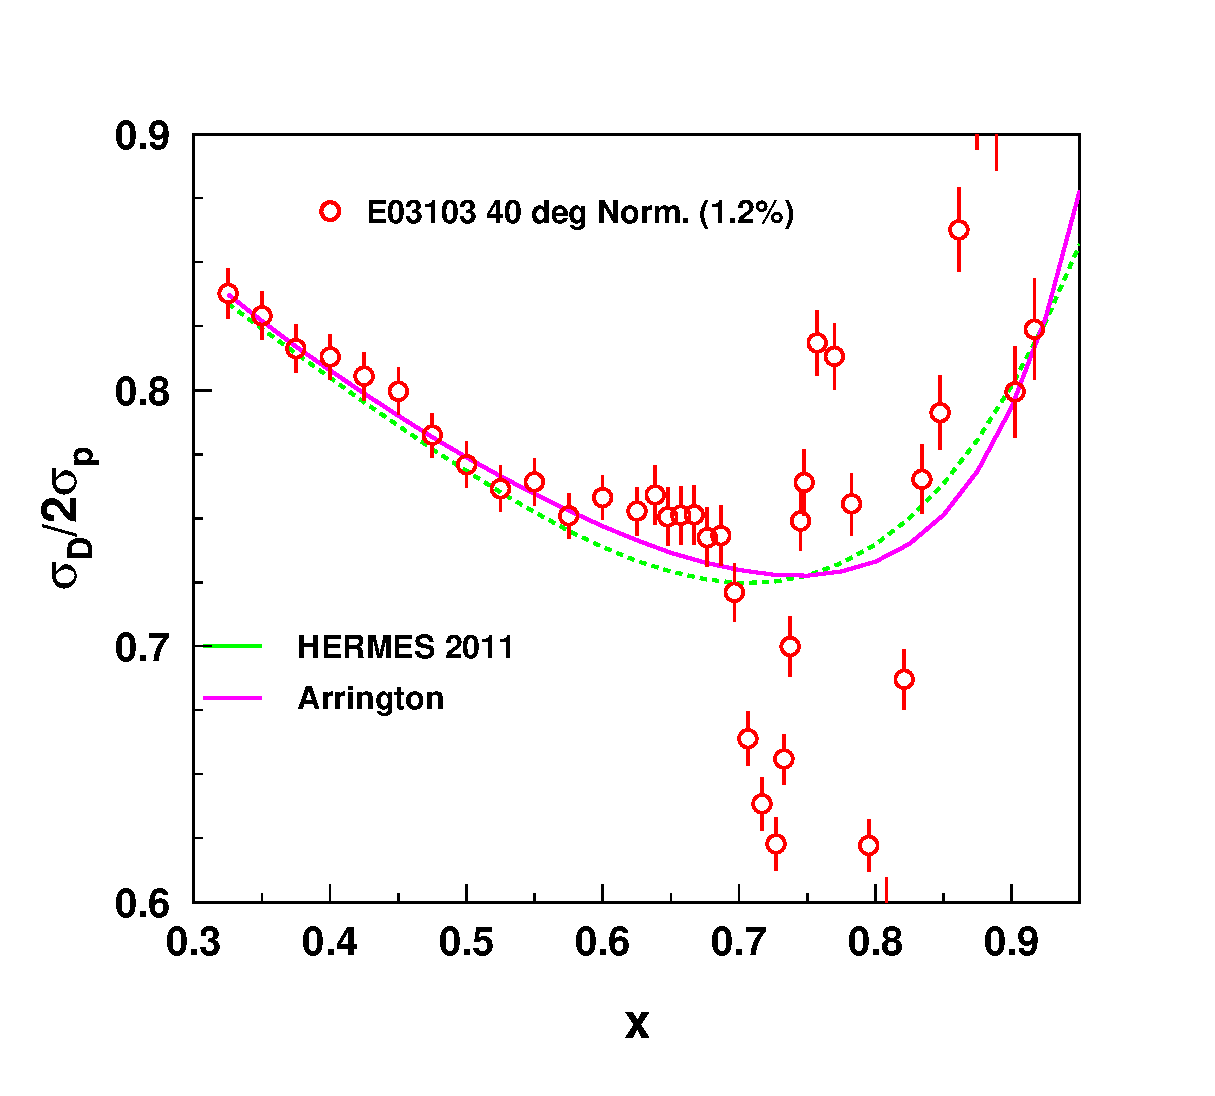
\includegraphics[height=65mm,angle=0]{plots/compare_dbyp_032012.eps}
\caption{Our extracted $\sigma^D/2\sigma^p$ ratio along with 
calculations based on different $F_2^n/F_2^p$ extractions (dashed line
from~\cite{hermes_dbyp} and solid line using~\cite{arrington09, arrington12b}.
The structure above $x \approx 0.65$, is mainly due to the resonance in the
proton structure function.
\label{dprat_fig}}
\end{center}
\end{figure}

In our analysis we make a modified isoscalar correction. Instead of using
free proton and neutron structure functions, we have used the contributions of
$F_2^p$ and  $F_2^n$ in $^2$H (i.e., $\overline{F_2^n}$ and
$\overline{F_2^p}$) in the above equation to correct the nuclear cross
sections.  As such, we are converting the deuteron structure in the 
denominator to a non-isoscalar deuteron, with the same $Z/N$ ratio as the
nucleus.  The alternative would be to evaluate the neutron-to-proton ratio
for all nuclei, which would involve significantly larger model dependence
in heavier nuclei.  In addition, we use the $n/p$ ratio at the kinematics of
our experiment, rather than taking the result from a high-$Q^2$ analysis.
We determine the in-deuteron $n/p$ ratio following the approach of
Refs.~\cite{arrington09, arrington12b}.  The extraction was performed 
taking the average of the values obtained using the different NN potentials
and off-shell effects evaluated in Ref.~\cite{arrington12b}, using the
calculated value of $\overline{F_2^p}$ in the deuteron, and taking
$\overline{F_2^n}/\overline{F_2^p} = (F_2^d -
\overline{F_2^p})/\overline{F_2^p}$. This does not involve removing the
nuclear effects to extract the free neutron structure function, as is 
usually the case, and so this procedure is somewhat less model dependent
than the extraction of the free $F_2^n/F_2^p$ ratio.  We note that these
analyses also demonstrated that the model-dependence is smaller than assumed
in some previous comparisons, as some previous extractions evaluated nuclear
effects at different $Q^2$ values than the data that was used to extract
$F_2^n/F_2^p$.  A similar result was seen in the analysis of the impact of
nuclear effects on the extraction of the proton pdfs~\cite{accardi11}.

%The goal of the isoscalar corrections are to  correct the data on the heavy
%target for the difference between the measured nucleus, \textit{e.g.} 26
%proton and 30 neutrons for iron, and an isoscalar nucleus with the same mass. 
%Therefore, one should be using proton and neutron structure functions at
%kinematics of the experiment, as one is correcting the cross sections measured
%at those kinematics. \textit{(aji: since we use D2 smearing now, not sure
%whether to mention the following  Besides, if  we are correcting the nuclear
%cross sections then we should be using the contributions of $F_2^p$ and 
%$F_2^n$ to the nuclear structure function instead of using the free proton
%and neutron structure functions)}. E03-103 results are extracted using global
%fits of free proton and neutron cross sections and broadened using  the
%$F_2^n/F_2^p$ ratio and the convolution procedure mentioned in
%\cite{arrington09}. These distributions are then used to get the bound
%$F_2^n/F_2^p$ ratios in nuclei. 


Figure~\ref{dprat_fig} shows the  $\sigma^D/2\sigma^p$ cross section ratios
extracted from the E03-103 data for the 40 degree kinematics. Representative
extractions~\cite{hermes_dbyp, arrington12b}, of the same ratio is also shown
in the figure. It should be noted that the isoscalar corrections depends on
$Q^2$, and this effect is not negligible at large $x$. The correction factors
derived using various parameterizations for $^3$He and Au are shown in
Figure~\ref{f2nf2psize_fig}.

\begin{figure}[htbp]  
%\begin{minipage}[htbp]{2.75in}% start figure a)
%\includegraphics[height=60mm, angle=0]{plots/f2nf2p_size_he3.eps}
%\end{minipage}
%\hfill
%\begin{minipage}[htbp]{2.75in}	% start figure b)
%\includegraphics[height=60mm,angle=0]{plots/f2nf2p_size_au.eps}
%\end{minipage}
\includegraphics[height=55mm,width=0.44\textwidth,clip]{plots/f2nf2p_size_he3.eps} \\
\includegraphics[height=55mm,width=0.44\textwidth,clip]{plots/f2nf2p_size_au.eps}
\caption{Magnitude of isoscalar corrections for $^3$He (top figure) and Au
(bottom figure) targets for the 40 degree data for the different
parameterizations of $F_2^n/F_2^p$ as discussed in the text. The solid black
line represents the multiplicative correction factors obtained using the
smearing method discussed in the text and was used in the E03-103 analysis
for the EMC ratio extraction.
\label{f2nf2psize_fig}}
\end{figure}

In the case of $^3$He, one can avoid the uncertainty associated with the
isoscalar corrections by extracting the ratio of $^3$He to ($^2$H+$^1$H).
This ratio and the comparison to the isoscalar-corrected $^3$He/$^2$H ratio
are presented in section~\ref{xdepresult.ssec}.


\subsection{Scaling violation effects at high $x$}\label{hixcor.ssec}

%The DIS structure functions give information about the momentum distribution
%of quarks in the nucleus. Within the quark parton model, the structure 
%function relates to the parton momentum distributions in the limit of
%large $Q^2$ and $\nu$.  

As discussed in Sec.~\ref{kinem.ssec}, deviations from the scaling of the
simple quark parton model arise due to QCD evolution of the pdfs, target-mass
corrections which involve to finite-$Q^2$ corrections to the approximations
made in the infinite $\nu$, $Q^2$ limit, and higher twist contributions which
go beyond incoherent scattering from individual partons.


%At finite $Q^2$ additional deviations from this picture can be important:
%so-called ``target-mass'' corrections which relate to terms which are
%neglected in the infinite $\nu$, $Q^2$ limit and higher-twist contributions
%which go beyond incoherent scattering from individual partons.  Note that the
%logarithmic evolution of the structure functions that arises in QCD also leads
%to scaling violations, but does not break the connection between the structure
%function and the quark distributions; it simply encodes the scale dependence
%of the pdfs in QCD. At large $x$ and  at finite $Q^2$, additional scaling
%violations can originate from resonance contributions. In the case of nuclei
%at very large $x$, quasi-elastic scattering from a nucleon in the nucleus,
%rather than scattering off of a single quasi free quark can  cause additional
%scaling violations.

%Though the  quark parton model is a simple formalism which helps to understand
%the qualitative features of  DIS data, it fails to explain the observed
%scaling violations. The formal basis to understand the scaling of structure
%functions (and the violations)  is through the operator product expansion
%(OPE) and renormalization group equations in  QCD.

%At large $Q^2$, QCD predicts a logarithmic dependence of  $Q^2$ for
%$F_2(x,Q^2)$. In addition to the logarithmic  scaling violations, at low
%$Q^2$, there are corrections called power corrections of the form
%$\mathrm{O}\left([1/Q^2]^n\right)$. One type of power correction  due to the
%non-vanishing mass of the target hadron and known as target mass corrections.
%This corrections arise purely from the kinematic effects associated with the
%finite values of  $Q^2/\nu^2=4x^2M^2/Q^2$ and hence falls off  like $M^2/Q^2$
%\cite{tarmasscor}. Another correction  is  sensitive to multi-parton
%co-relations in the target (dynamical corrections), and with in the twist
%expansion of operators, these are associated with higher twists (in the OPE,
%the twist of an operator is defined as its free field dimension minus spin).
%The definition of $x$ as the light-cone momentum carried by the interacting
%parton is only valid in the massless target and quark limits and at finite
%value of  $Q^2$ these effects modify the interpretation of $x$ as light cone
%momentum fraction~\cite {Schienbein_tarmass_rev}. Thus, in the region where
%W$\rightarrow$M, these kinematical and dynamical higher twist corrections
%need to be considered.

The kinematic effects due to target mass corrections were first calculated in
the framework of the operator product expansion OPE by~\cite{georgi_tmc}.  In
the nucleon case, the measured structure function $F_2^{meas}$ can be related
to the massless limit structure function $F_2^{(0)}$~\cite
{Schienbein_tarmass_rev} via
%
\begin{eqnarray} \nonumber  \label{tarmass_eqn}
F_2^{meas}(x,Q^2)&=&\frac{x^2}{\xi^2 r^{3}}F_2^{(0)}(\xi,Q^2) + \frac{6M^2x^3}{Q^2 r^{4}}h_2(\xi,Q^2)\\
&& +\frac{12M^{4}x^4}{Q^{4} r^{5}}g_2(\xi,Q^2)
\end{eqnarray}
%
where $h_2(\xi,Q^2) =\int_{\xi}^{1}du~u^{-2} F_2^{(0)}(u,Q^2)$, $g_2(\xi,Q^2)
=\int_{\xi}^{1}dv~(v-\xi)v^{-2} F_2^{(0)}(v,Q^2)$, $r=\sqrt{1+\frac{Q^2}{
4x^2M^2}}$ and $\xi = \frac{2x}{1+r}$. $F_2^{(0)}$ do not contain target mass
effects and this is the function which obeys the QCD evolution effects in the
absence of higher twist effects. It should be noted that there are different
prescriptions~\cite {Schienbein_tarmass_rev, Accardi_tarmass2008plb,
Accardi_tarmass2008jhep} available for these kinematical corrections with
slightly different end results, however, the appropriate prescription for
target mass corrections in nuclei is not well defined.

For the extraction of EMC effect we are looking at the A/D ratios of the
measured cross sections, so any A-independent scaling violations will cancel
in the ratios. If the $h_2$ and $g_2$ corrections are negligible or target
independent, then $F_2^{meas}(x,Q^2)$ is directly connected to
$F_2^{(0)}(\xi,Q^2)$ (see Eqn~\ref{tarmass_eqn}) through a simple relation. In
that case, the target mass effects on cross section ratios can be well
approximated by $x\rightarrow \xi$ substitution. Our investigations show that
the $h_2$ and $g_2$ terms yield corrections $\ltorder$ 5\% to the structure
functions for $Q^2$ $>$ 5 GeV$^2$~\cite{nadia_f2prl} and for E03-103, $Q^2$
values are greater than 5 GeV$^2$ for the 40 and 50 degree data above $x$=0.7.
In the ratio, the impact is further suppressed.  \textit{WHAT ABOUT $Q^2$
VALUES BELOW 5 GEV$^2$ ($x<0.7$)?}

Higher-twist effects can also lead to scaling violations, although it has been
argued based on quark-hadron duality~\cite{niculescu00a, melnitchouk:2005zr}
that for nuclei, the Fermi motion of the nucleons samples a sufficient
kinematic region that the observed structure function reproduces the DIS limit
even down to extremely low $Q^2$ and $W^2$ values~\cite{Arrington:2003nt}. 
This will be examined with the extensive measurements taken
to examine the $Q^2$ dependence of the EMC ratio.

%Experimental evidence for the lack of $Q^2$ dependence arising from these
%corrections can be found in Fig.~\ref{emc_x_C_hiq2dep_fig}. This figure shows
%the $Q^2$ dependence of the EMC ratios for C as a function of $x$. The $Q^2$
%values varies from 4.06 to 6.05 at $x=0.75$. This varies from 4.50 to 6.91 at
%$x=0.9$. Note that both higher twist and target mass corrections are $1/Q^2$
%power corrections. Even at higher $x$ values there was no indication of a
%clear $Q^2$ dependence within the available statistics.


\begin{figure}[htb]
\begin{center}
\includegraphics[width=80mm,angle=0]{plots/qe_contri.eps}
\caption{Fractional quasielastic contribution to the cross section based on
our model at 40 degrees for $^2$H, $^{12}$C and $^{197}$Au. Here,
$\sigma_{qe}$ is the contribution from the quasielastic piece of the model
(in the Born approximation) and $\sigma_{Born}$ is the total Born cross section.
\label{qe_contri_fig}}
\end{center}
\end{figure}

It is unclear if the extended scaling of the EMC ratio will hold true in the
presence of significant contributions from quasielastic
scattering~\cite{melnitchouk:2005zr, niculescu06, Osipenko:2010sb}. 
Figure~\ref{qe_contri_fig} shows the quasielastic contribution,
$\sigma_{qe}/\sigma_{Born}$, based on our cross section model for the 40
degree kinematics.  In our model, the quasielastic contribution is negligible
for $x \ltorder 0.7$, and $\ltorder$10\% for all nuclei up to $x=0.9$, with
further suppression when examining target ratios. 
